
\chapter{Implementace a testování metod}
\label{chap:impl}

Praktická část práce se zabývá porovnáním výkonnosti metod nalezení a popisu bodových příznaků na použitém datasetu. Je stanovena metrika výkonnosti a kombinace metod jsou testovány na výkonnost, rychlost detekce a počet nalezených bodů na celém datasetu a jeho částech.

\section{Dataset}

\begin{figure}[!ht] 
	\centering
	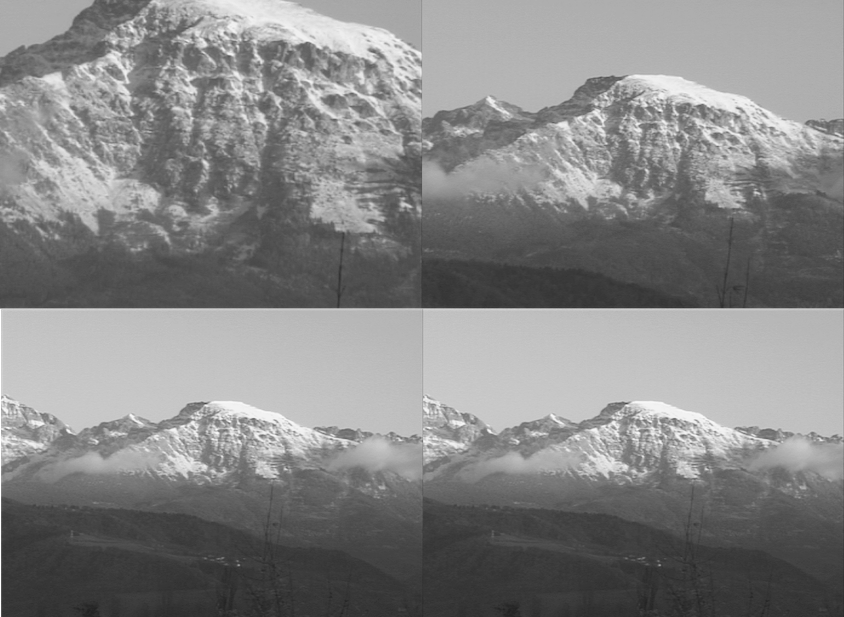
\includegraphics[width=5in]{img/belledonne.png}
	\caption{Subset Belledonne z datasetu - stejná scéna s postupně se zmenšujícím zoomem. Porovnává se vždy první obrázek vlevo nahoře s jedním z ostatních } 	\label{dataset_belledonne}
\end{figure}

Pro experimenty v této práci byl použit dataset volně dostupný na webu \footnote{\url{http://kahlan.eps.surrey.ac.uk/featurespace/web/related_papers/affine.html}}. Všechny datasety na tomto webu byly prozkoumány skriptem \verb|create_configs.py| a byly z nich vytěženy všechny páry obrázků, ke kterým je zadána zároveň matice homografie (viz sekce \ref{sec:homo}). Výsledný dataset sestává z jednotlivých subsetů obsahujících vždy několik obrázků zobrazujících jednu scénu pod různými prostorovými transformacemi. Příkladem je subset Belledone na obrázku \ref{dataset_belledonne}, nebo subsety Monet a Asterix, jejichž vždy jeden vybraný pár je vidět na obrázcích \ref{ex_MONET} a \ref{ex_asterix}. Dále byly z této množiny vytvořeny subsety podle transformace, která se v nich odehrává. Některé subsety obsahují skutečnou prostorovou transformaci, tj. rotaci podle osy procházející středem fotoaparátu (subset rot), změnu úhlu pozorování (angle), nebo zoom, jiné jsou téměř nebo zcela statické a testují robustnost detektorů a deskriptorů vůči jiným transformacím: rozostření(blur), změnám světelných podmínek (light) nebo změně rozlišení obrazu(res). Porovnává se vždy jeden z obrázků s postupně všemi ostatními (obr. \ref{dataset_belledonne}). 

\section{Homografie}
\label{sec:homo}

Homografie \cite{berenda2010homografie}, nebo také projektiní transformace je invertibilní transformacemezi dvěma projektivními pohledy (tzn. pohledy například fotoaparátu do 3D scény). Přímce z jednoho pohledu přiřazuje vždy přímku v druhém pohledu, bodu přiřazuje bod. Vyjadřuje tedy, jak se mění vjem pozorovaného předmětu v závislosti na změnách pozice, rotace nebo úhlu pohledu pozorovatele. Homografie je popsána transformační maticí $\mathbb{H}$ o rozměru $3\times 3$. Pro transformaci bodu z jedné projektivní plochy na druhou $x_i \leftrightarrow x'_i$ platí:
\begin{equation}
x'_i = \mathbb{H}x_i = 
\begin{bmatrix}
h_{11} & h_{12} & h_{13} \\
h_{21} & h_{22} & h_{23} \\
h_{31} & h_{32} & h_{33}
\end{bmatrix}
\begin{bmatrix}
x_i \\ y_i \\ 1
\end{bmatrix}
= 
\begin{bmatrix}
x'_i \\ y'_i \\ w'_i
\end{bmatrix},
\end{equation} 
kde souřadnice $w'$ představuje měřítko. Matici homografie lze potom nalézt spojením těchto rovnic pro asociované páry nalezených bodů ve zdrojových obrazech a aproximací řešení přeurčené soustavy rovnic například metodou nejmenších čtverců nebo RANSAC. 

Vzdálenost deklarované a nalezené homografie je v experimentech této práce brána jako měřítko kvality konkrétní metody nebo kombinace metod na daném datasetu. Kvalita homografie nabývá hodnot od 0 do 100\% a vypočítává se jako:

\begin{align}
	pi_1 = H_1 * eig(H_1) \\
	pi_2 = H_2 * eig(H_2) \\
	dif = pi_1 - pi_2 \\
	100*(\frac{pi}{2} - atan(dif \times{} 10^-4))
\end{align}

kde $H_1$ je homografie deklarovaná v datasetu, $H_2$ je matice homografie nalezená
programem, $eig(H)$ jsou vlastní čísla matice $H$. 

%Dále je zkoumán celkový počet přiřazených bodů (označen 'matches') a z něj počet bodů použitých k aproximaci homografie (označen 'inliers'). Dále jsou zkoumány časy pro detekci a popis při použití jednotlivých detektorů a deskriptorů. 

%IMPLEMENTACE

\section{Implementace}

\begin{figure}[!htp] 
	\centering
	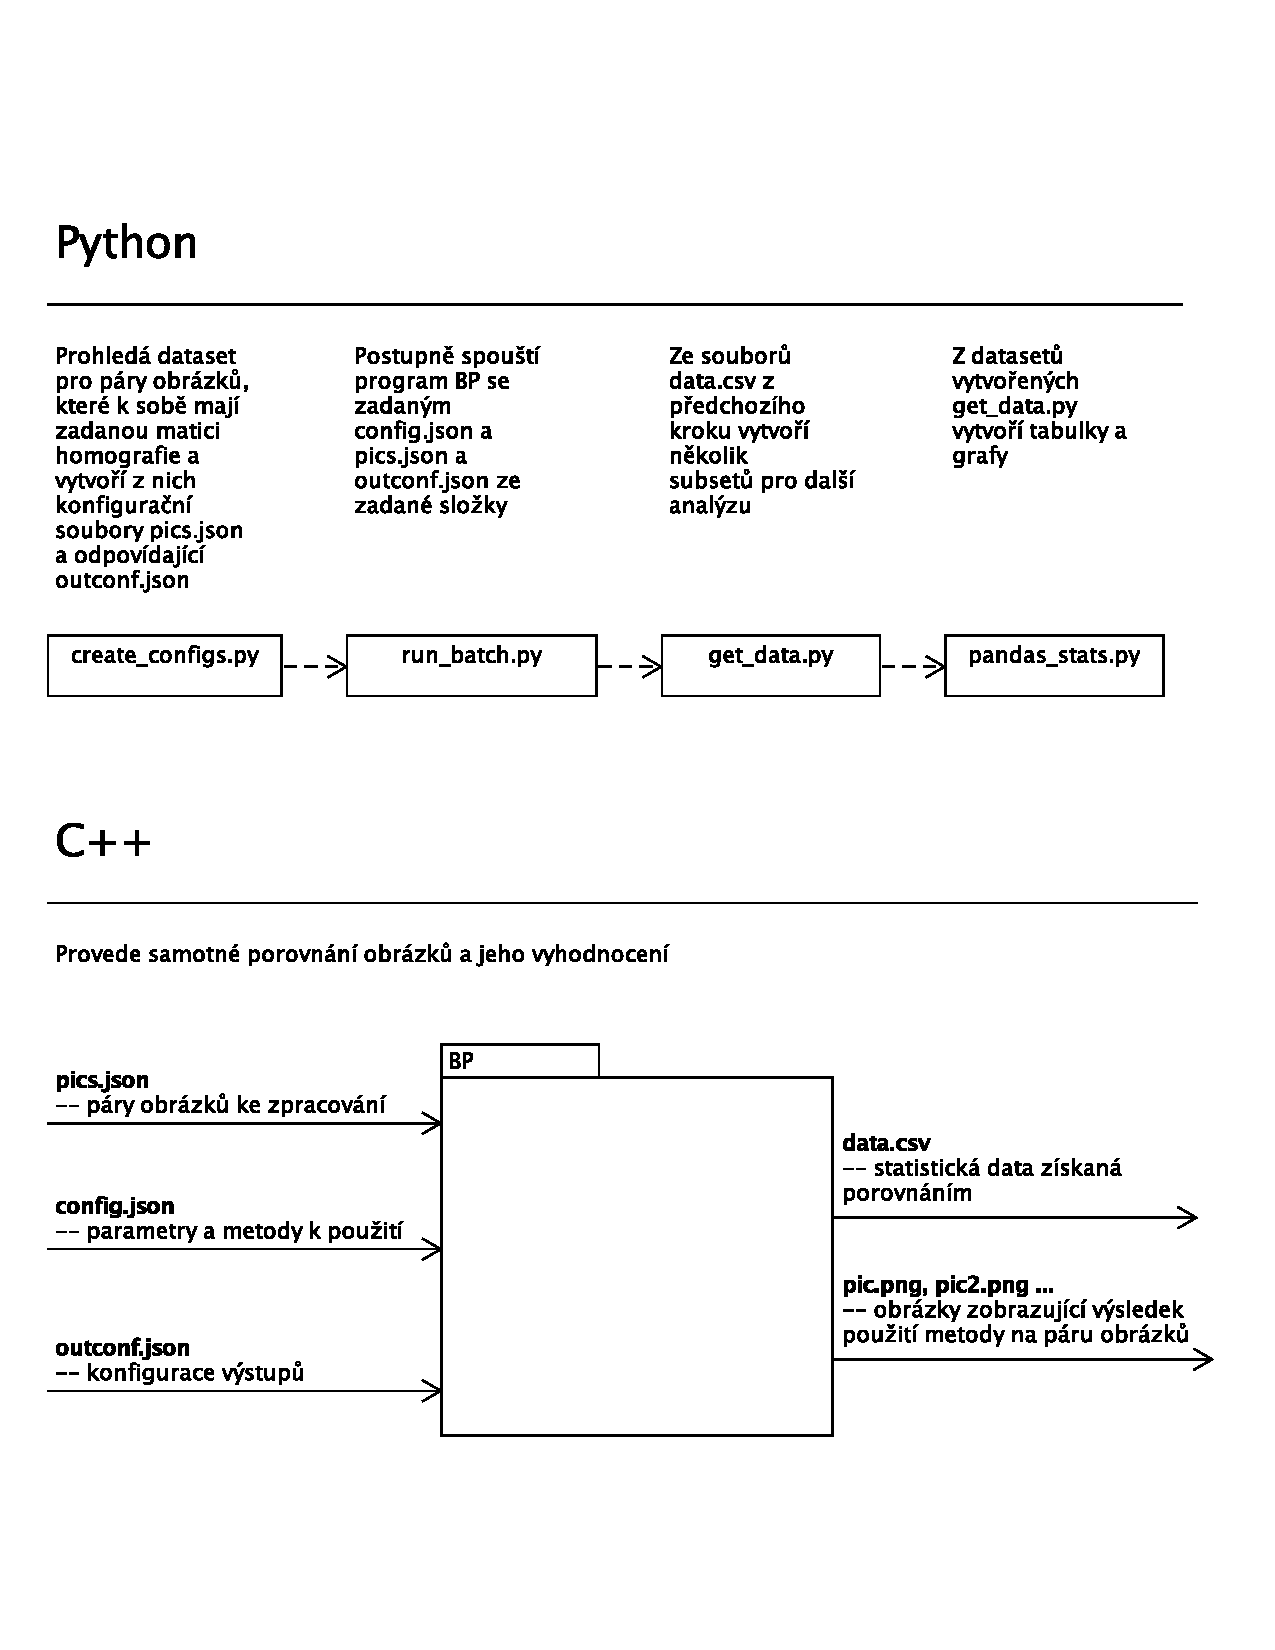
\includegraphics[width=6in]{img/impl_uml.pdf}
	\caption{Schema implementace programů provádějících experimenty a jejich vyhodnocení} \label{impl_uml}
\end{figure}

Porovnání jednotlivých metod bylo implementováno v hlavním programu v C++ s využitím frameworku openCV. Zpracování datasetu, dávkové spouštění porovnání a statistické vyhodnocení výsledků bylo implementováno v jazyku Python s využitím knihovny Pandas. Schema implementace lze vidět na obrázku \ref{impl_uml}. Celá implementace společně se zdrojovými soubory pro tento dokument je k nalezení na githubu autora \footnote{\protect\url{https://github.com/PetrBarborka/BPrace}}

Data o souborech v datasetu jsou vytěžena skriptem \verb|create_configs.py| v Pythonu a zkompilována do konfiguračních souborů pro hlavní program \verb|BP|. Skript \verb|run_batch.py| poté tyto konfigurační soubory načte a postupně s nimi spustí hlavní program. Ten pro každou vybranou složku datasetu vytvoří výstupní složku s obrázky, které zobrazují nalezené a spojené body mezi jedním a druhým obrázkem z vyhodnocovaného páru a soubor \verb|data.csv|, který obsahuje informace o jednotlivých párech, rychlostech vyhodnocení a kvalitě odhadu homografie. Skript \verb|get_data.py| ze souborů \verb|data.csv| vytvoří jeden globální soubor a několik souborů se subsety podle transformace, kterou reprezentují: Úhel (ve smyslu změna polohy pozorovatele směrem do stran), rotace (okolo osy procházející středem fotoaparátu), zoom, nasvětlení, rozostření a změna rozlišení. Tyto soubory jsou zpracovány skriptem \verb|pandas_stats.py| do obrázků a tabulek v této kapitole.

Hlavní program sestává ze čtyř tříd. První tři zajišťují obalení detektorů, deskriptorů a nástrojů výpočtu homografie z openCV tak, aby spolu všechny varianty vzájemně fungovaly a aby byly jednotlivé metody implementačně zaměnitelné. Poslední třída zajišťuje servisní funkce jako vstup a výstup a podobně. Tyto třídy jsou využity v hlavním souboru main.cpp, který zpracuje vstupní argumenty z příkazového řádku a spustí příslušné procesy. K práci s formátem json je využita knihovna Nielse Lohmanna (\url{https://github.com/nlohmann/json}).

Pythonové skripty procházejí sobourový systém pomocí \verb|os.walk()| a vytvářejí a čtou soubory. Ve skriptu \verb|run_batch.py| je k dávkovému spouštění programu \verb|BP| použit modul subprocess, který umožňuje spustit libovolné množství instancí paralelně. Skript \verb|pandas_stats.py| k práci s databází výsledků používá statistickou knihovnu Pandas.

\section{Experimenty}

Na datasetu jsou zkoumány detektory příznakových bodů Harris, GFTT (neboli Shi-Tomasi), SIFT, SURF, FAST, ORB a MSER a deskriptory BRIEF, SIFT, SURF a ORB. Body nalezené a popsané těmito algoritmy jsou potom mezi jednotlivými obrazy přiřazeny a metodou na bázi RANSAC je z nich aproximována matice homografie. Jsou označeny body (páry bodů), které byly pro tuto aproximaci vzaty jako správné a ty,  které byly zavrženy jako chybně přiřazené.

\begin{figure}[!ht] 
	\centering
		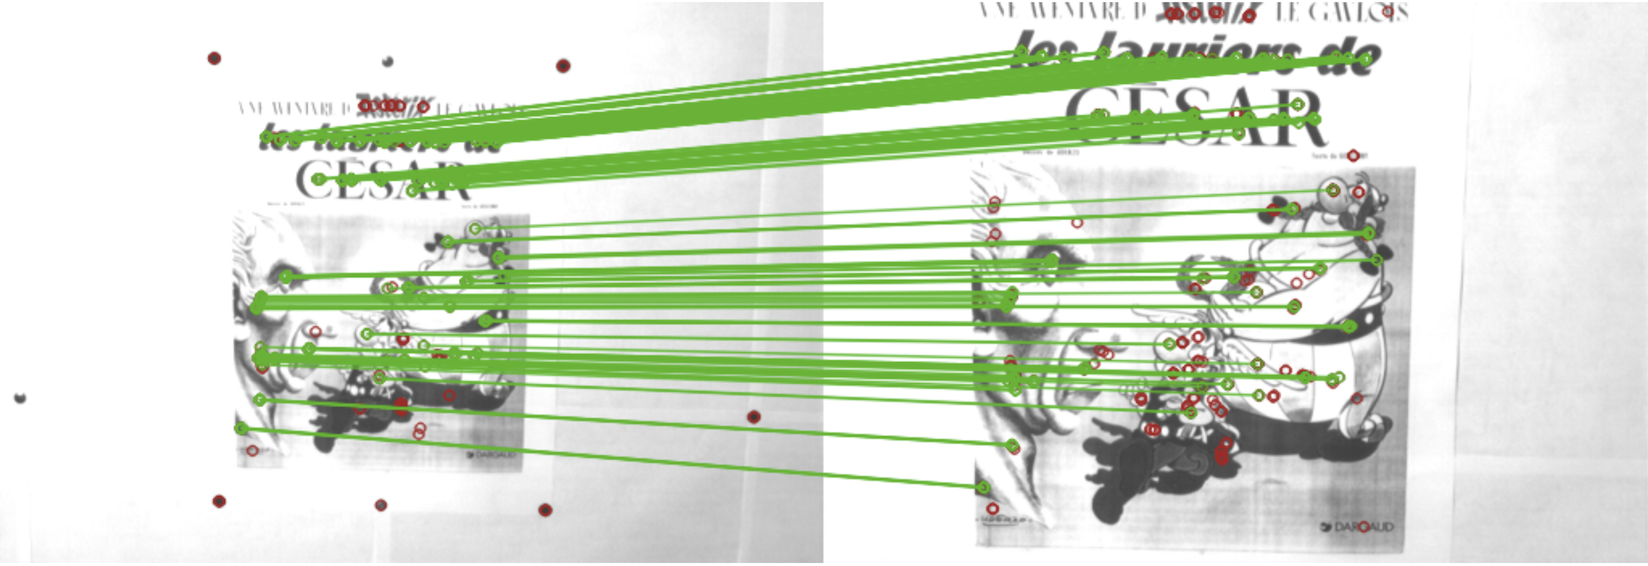
\includegraphics[width=5in]{img/ex_ASTERIX_MSER_SIFT.png}
	\caption{Transformace zoom ze subsetu Asterix, detektor MSER,
		deskriptor SIFT} \label{ex_asterix}
\end{figure}

\begin{figure}[!ht] 
	\centering
		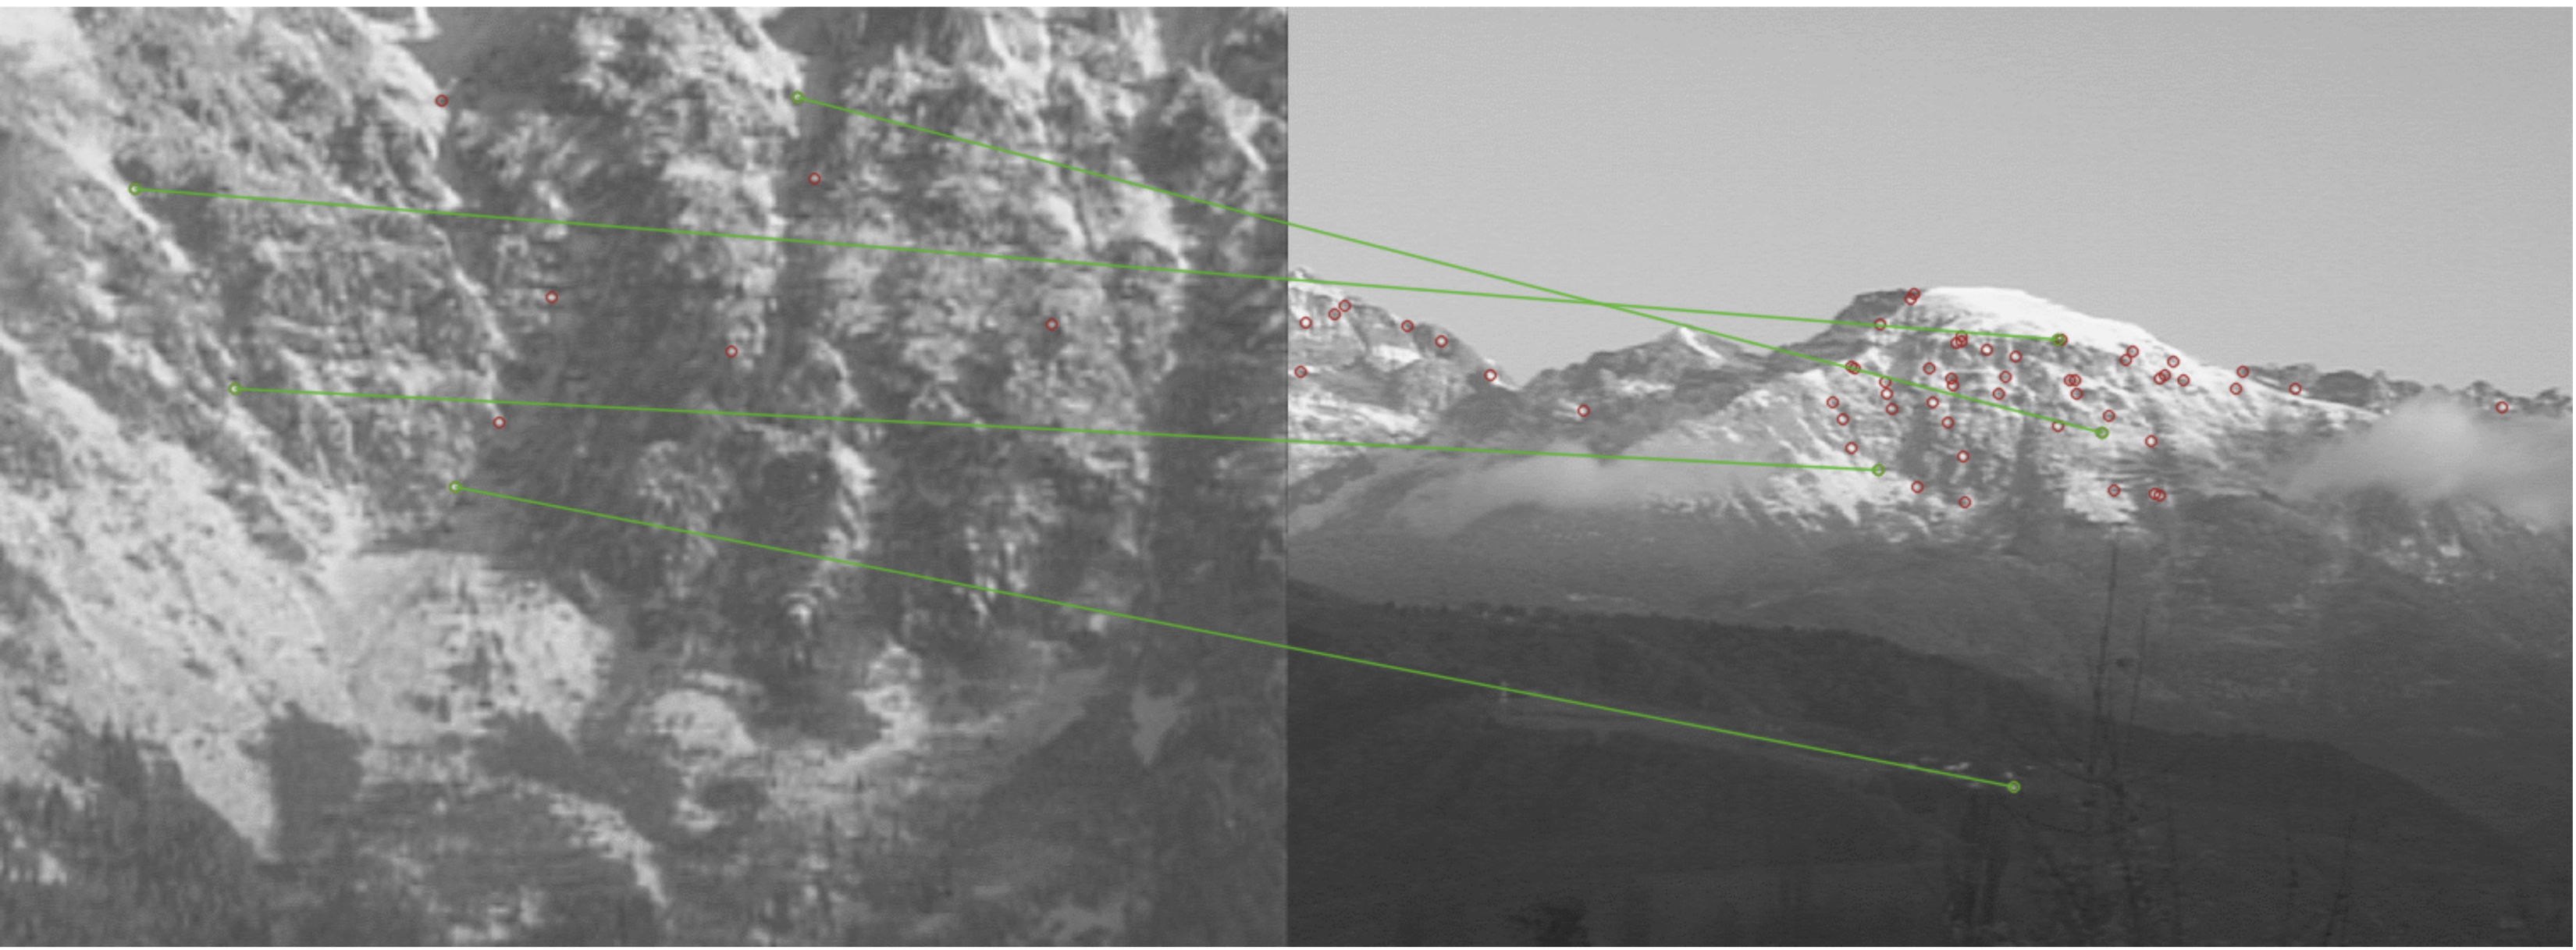
\includegraphics[width=5in]{img/ex_BELLEDONNE_FAST_ORB.png}
	\caption{Ukázka transformace zoom ze subsetu Belledonne, detektor FAST,
		deskriptor ORB}	\label{ex_belledonne}
\end{figure}

\begin{figure}[!ht] 
	\centering{
		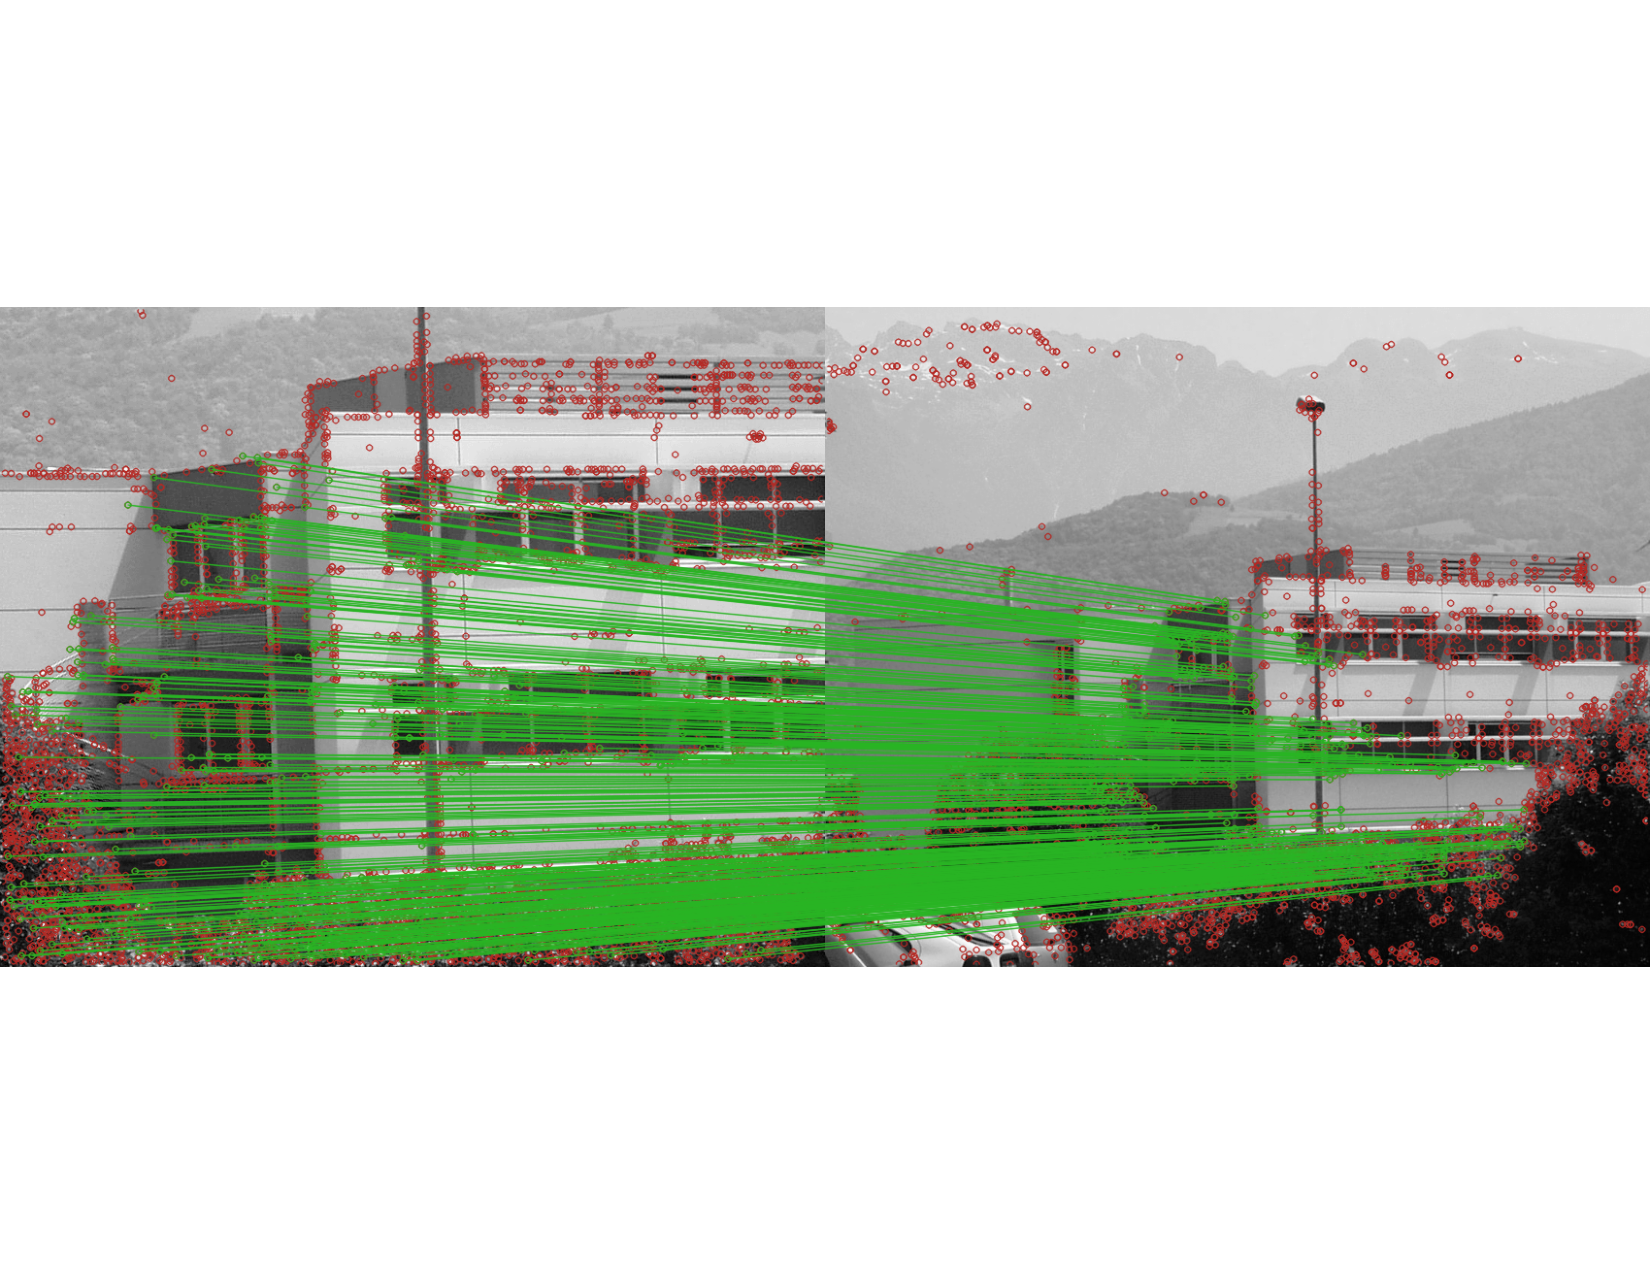
\includegraphics[width=5in]{img/ex_ENSIMAG_SIFT_SIFT.png}}
	\caption{Ukázka transformace zoom ze subsetu Ensimag, detektor i 
		deskriptor SIFT} \label{ex_ensimag}
\end{figure}

\begin{figure}[!ht] 
	\centering{
		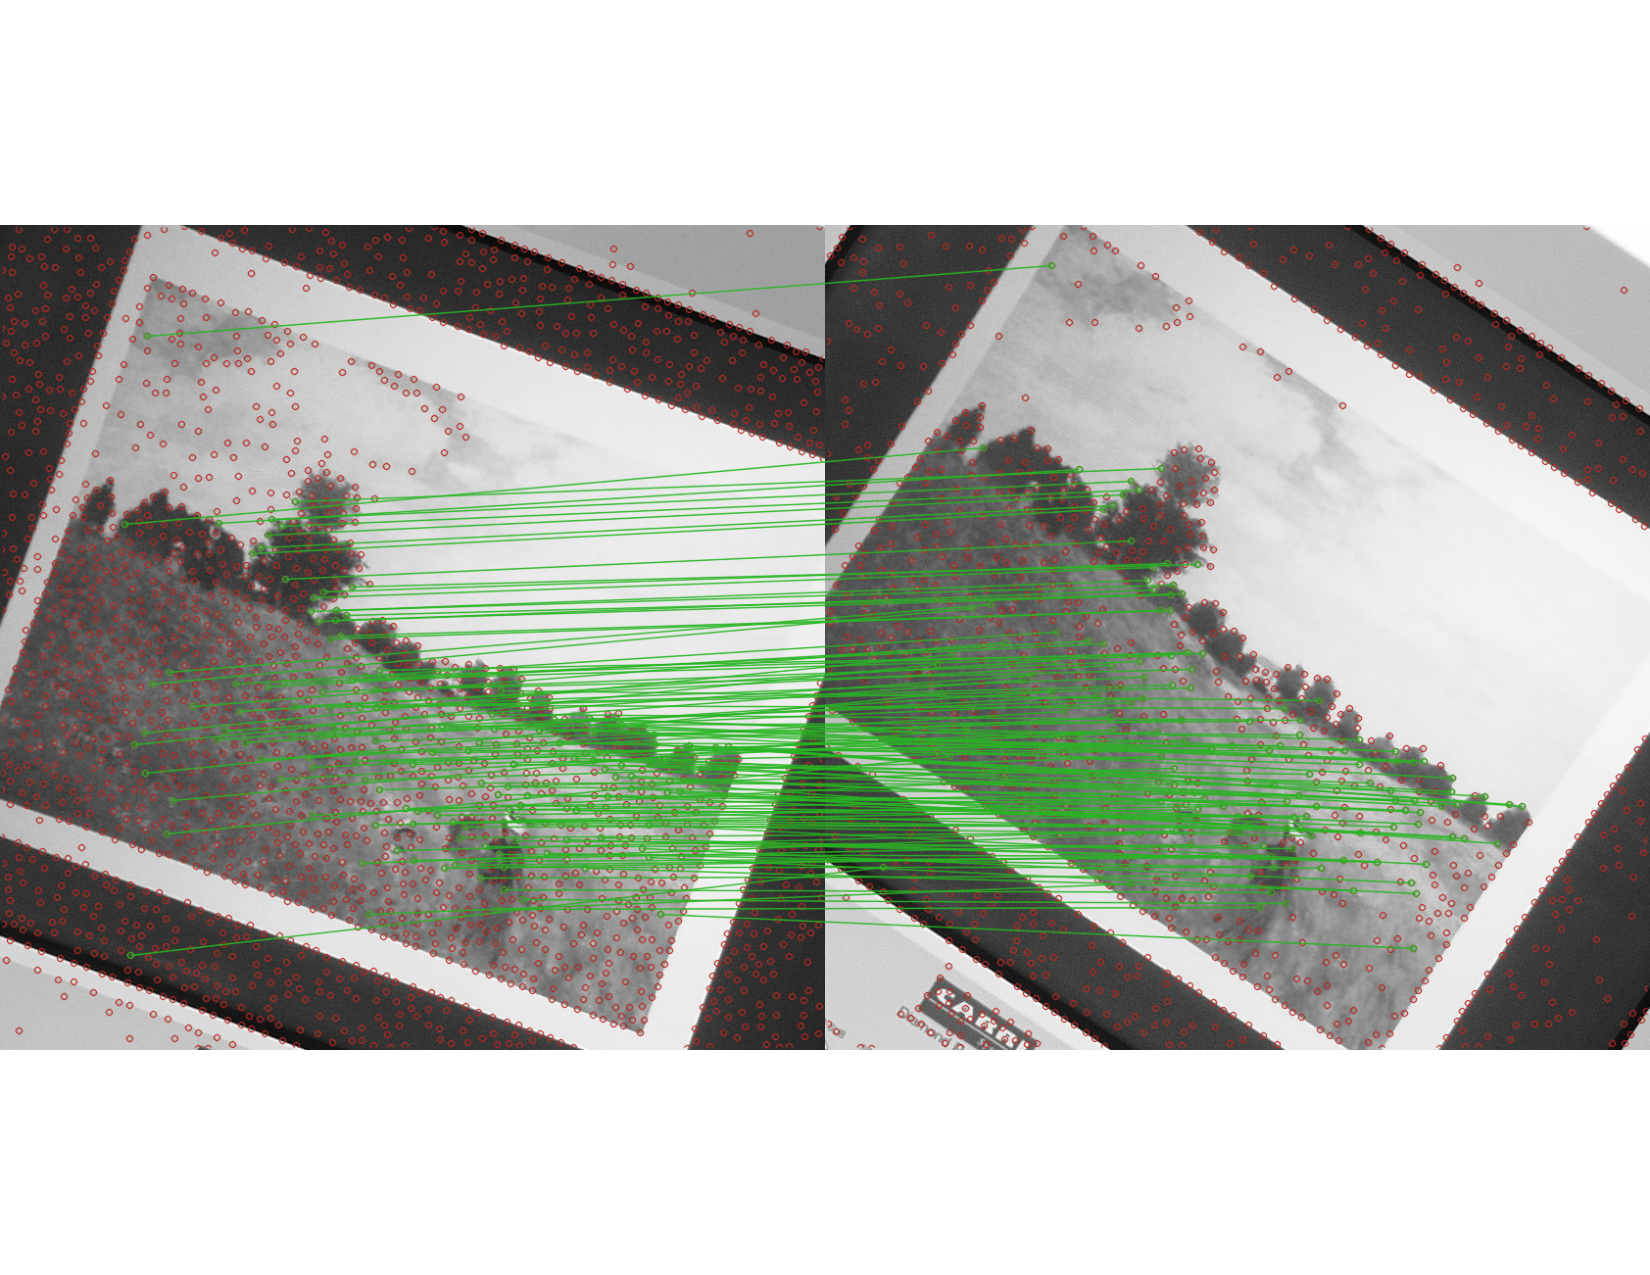
\includegraphics[width=5in]{img/ex_MONET_GFTT_SIFT.png}}
	\caption{Ukázka transformace rotace ze subsetu Monet, detektor GFTT, 
		deskriptor SIFT} \label{ex_MONET}
\end{figure}

V tabulkách \ref{tab_detperf} a \ref{tab_descperf} je uveden přehled celkových průměrných výkonností jednotlivých deskriptorů a detektorů. Tento přehled je získán vždy testováním uvedeného subsetu uvedenou metodou a všemi metodami z druhé kategorie. Tedy například skóre deskriptoru SURF je průměrem kombinace deskriptoru SURF a všech testovaných detektorů na daném datasetu. Jak je vidět v \ref{tab_detperf}, v celkové výkonnosti vede detektor ORB. Při bližším pohledu vidíme, že exceluje zejména na subsetech blur (rozostření), light (změna světelných podmínek) a res (změna rozlišení). Z toho lze usoudit, že tento detektor založený na algoritmu FAST je vůdči těmto změnám parametrů obrazu velmi robustní. Za povšimnutí stojí, že jeho varianta - samostatná implementace algoritmu FAST v openCV má na všech subsetech asi poloviční hodnocení. Z toho je zřejmé, že se výkonnost detekčního algoritmu může drasticky změnit drobnými úpravami parametrů a vylepšeními aniž by se změnil jeho princip. Detektor SURF ve všech disciplínách překonal SIFT, přestože vznikl jako jeho aproximace.

\begin{table}[!ht]\centering
\begin{tabular}{ l| r r r r r r r }
	Detektor & celkově[\%] & zoom[\%] & blur[\%] & rot[\%] & angle[\%] & light[\%] & res[\%] \\
	\hline
	 Harris & 25.21 & 15.94 & 54.14 & 30.84 & 19.60 & 58.23 & 53.75 \\
	 GFTT & 24.18 & 16.83 & 49.85 & 30.33 & 18.95 & 55.30 & 45.88 \\
	 SIFT & 32.27 & 24.88 & 25.83 & 42.82 & 21.83 & 46.74 & 35.94 \\
	 SURF & 38.01 & 30.66 & 50.87 & 47.03 & 25.74 & 51.27 & 52.41 \\
	 FAST & 22.67 & 11.34 & 13.55 & 30.80 & 19.55 & 56.18 & 42.21 \\
	 MSER & 32.07 & 30.54 & 50.49 & 34.48 & 26.88 & 59.94 & 65.58 \\
	 ORB & 49.91 & 27.86 & 74.76 & 66.96 & 34.31 & 77.05 & 75.53
\end{tabular}
	\caption[Short Heading]{\protect Celková výkonnost detektorů na datasetech}\label{tab_detperf}
\end{table}

Ve srovnání deskriptorů (tabulka \ref{tab_descperf}) naopak ORB, založený na algoritmu BRIEF zaostává nad svou samostatnou implementací. Jako deskriptor má SIFT nad SURF převahu ve statických scénářích (subsety blur, light, res).

\begin{tabular}{ l| r r r r r r r }
\label{tab_descperf}
	desc method & total score [\%] & zoom score [\%] & blur score [\%] & rot score [\%] & angle score [\%] & light score [\%] & res score [\%] \\
	\hline
	 BRIEF & 13.55 & 9.39 & 14.14 & 17.77 & 9.68 & 19.78 & 22.63 \\
	 SIFT & 48.52 & 41.48 & 93.01 & 54.24 & 40.40 & 99.53 & 99.94 \\
	 SURF & 59.85 & 33.52 & 70.14 & 82.66 & 40.96 & 96.61 & 82.54 \\
	 ORB & 5.93 & 5.81 & 1.25 & 6.78 & 4.08 & 14.24 & 6.17
\end{tabular}

Ze srovnání kombinací (tabulky \ref{tab_comboperf_static} a \ref{tab_comboperf_dynamic}) je zřejmé, že všechny detektory mají nejlepší výsledky v kombinaci s deskriptory SIFT a SURF.

\begin{table}[htbp]\centering
\begin{tabular}{ l l| r r r r r r r }
	Detektor & Deskriptor & celkově[\%] & zoom[\%] & blur[\%] & rot[\%] & angle[\%] & light[\%] & res[\%] \\
	\hline
	 Harris &  BRIEF & 4.05 & 6.87 & 2.23 & 2.64 & 4.20 & 11.70 & 3.10 \\
	 Harris &  SIFT & 29.76 & 27.06 & 97.58 & 27.58 & 25.96 & 99.51 & 99.96 \\
	 Harris &  SURF & 59.44 & 23.07 & 98.27 & 85.05 & 42.91 & 99.53 & 99.96 \\
	 Harris &  ORB & 5.37 & 5.67 & 1.16 & 6.32 & 2.77 & 12.88 & 1.83 \\
	 GFTT &  BRIEF & 6.43 & 7.51 & 1.70 & 6.78 & 8.46 & 12.68 & 2.20 \\
	 GFTT &  SIFT & 27.78 & 29.19 & 97.42 & 23.44 & 27.98 & 99.49 & 99.82 \\
	 GFTT &  SURF & 57.48 & 26.09 & 98.89 & 84.55 & 36.21 & 99.53 & 79.96 \\
	 GFTT &  ORB & 5.04 & 4.54 & 1.40 & 6.54 & 3.16 & 9.49 & 1.54 \\
	 SIFT &  BRIEF & 5.12 & 5.04 & 1.45 & 5.99 & 4.06 & 4.80 & 3.05 \\
	 SIFT &  SIFT & 74.55 & 60.97 & 99.48 & 88.76 & 57.16 & 99.52 & 99.90 \\
	 SIFT &  SURF & 44.17 & 27.33 & 0.98 & 70.25 & 23.61 & 79.18 & 37.37 \\
	 SIFT &  ORB & 5.25 & 6.19 & 1.41 & 6.28 & 2.49 & 3.46 & 3.44 \\
	 SURF &  BRIEF & 5.41 & 5.83 & 2.71 & 6.40 & 4.90 & 3.64 & 3.89 \\
	 SURF &  SIFT & 72.50 & 61.26 & 99.64 & 87.39 & 49.20 & 99.51 & 99.99 \\
	 SURF &  SURF & 69.15 & 51.04 & 99.62 & 87.98 & 45.67 & 99.51 & 99.80 \\
	 SURF &  ORB & 4.96 & 4.52 & 1.53 & 6.35 & 3.21 & 2.40 & 5.96 \\
	 FAST &  BRIEF & 4.68 & 3.95 & 2.28 & 5.91 & 2.56 & 3.60 & 2.25 \\
	 FAST &  SIFT & 32.24 & 26.34 & 49.85 & 32.96 & 38.64 & 99.53 & 99.96 \\
	 FAST &  SURF & 47.83 & 11.23 & 1.33 & 77.98 & 31.22 & 99.42 & 60.68 \\
	 FAST &  ORB & 5.93 & 3.84 & 0.74 & 6.36 & 5.80 & 22.17 & 5.96 \\
	 MSER &  BRIEF & 10.19 & 14.45 & 1.40 & 11.29 & 3.99 & 0.91 & 40.01 \\
	 MSER &  SIFT & 38.91 & 50.45 & 99.80 & 33.41 & 41.05 & 99.69 & 99.99 \\
	 MSER &  SURF & 69.33 & 45.26 & 99.64 & 83.92 & 53.92 & 99.59 & 99.99 \\
	 MSER &  ORB & 9.86 & 12.01 & 1.12 & 9.32 & 8.58 & 39.58 & 22.33 \\
	 ORB &  BRIEF & 58.42 & 21.80 & 99.76 & 85.56 & 38.69 & 99.52 & 100.00 \\
	 ORB &  SIFT & 64.27 & 35.07 & 99.54 & 87.06 & 42.82 & 99.46 & 99.96 \\
	 ORB &  SURF & 71.83 & 50.63 & 98.41 & 88.92 & 53.18 & 99.53 & 100.00 \\
	 ORB &  ORB & 5.11 & 3.92 & 1.32 & 6.32 & 2.56 & 9.67 & 2.15
\end{tabular}
	\caption[Short Heading]{\protect Celková výkonnost kombinací detektor -> deskriptor}\label{tab_comboperf}
\end{table}

Při aplikaci v reálném čase na frekvenci 20Hz je na jeden celý cyklus uvažovaného systému k dispozici 0.05 vteřiny. Uvažujeme-li, že systém musí v každém cyklu provádět i jiné operace než detekci a popis příznaků, můžeme počítat s 0.025 vteřiny pro obě operace dohromady. Časy v tabulkách \ref{tab_dettimes} a \ref{tab_desctimes} představují dobu potřebnou pro nalezení příznaků v obou obrazech z testovaného páru, náročnost na jednom obraze bude tedy zhruba poloviční. Do této periody by se podle získaných dat žádná z kombinací zkoumaných metod nevešla. To je pravděpodobně způsobeno nedokonalým nastavením parametrů jednotlivých metod, vysokým rozlišením zpracovávaných obrazů a vysokým množstvím detekovaných příznaků (nebylo nijak omezeno), protože všechny porovnávané metody již byly nějakým způsobem v systémech pracujících v reálném čase nasazeny.

Z porovnání časů potřebných k detekci a popisu příznaků v tabulkách \ref{tab_dettimes} a \ref{tab_desctimes} lze vidět, že SIFT a SURF platí za svoji výkonnost o řád delším časem detekce před ostatními s výjimkou MSER a dokonce o dva řády delším časem výpočtu deskriptorů.
\begin{tabular}{ l l }
	Detection method & avg det time [s] \\
	\hline
	 Harris & 0.05 \\
	 GFTT & 0.05 \\
	 SIFT & 0.82 \\
	 SURF & 1.00 \\
	 FAST & 0.00 \\
	 MSER & 0.80 \\
	 ORB & 0.08
\end{tabular}
\begin{tabular}{ l| r }
\label{tab_desctimes}
	Description method & avg desc time [s] \\
	\hline
	 BRIEF & 0.07 \\
	 SIFT & 8.23 \\
	 SURF & 2.97 \\
	 ORB & 0.07
\end{tabular}

Dle tabulky \ref{tab_matchcount} produkuje při daném nastavení největší množství příznaků detektor ORB. Lze ale také vidět, že množství detekovaných příznaků nemá přímou souvislost s kvalitou aproximace matice homografie.

\begin{table}[htbp]\centering
\begin{tabular}{ l l| r r r }
	Detektor & Deskriptor & průměrně párů & průměrně použitých párů & průměrné skóre [\%] \\
	\hline
	 Harris &  BRIEF & 482.16 & 11.40 & 4.05 \\
	 Harris &  SIFT & 554.30 & 84.87 & 29.76 \\
	 Harris &  SURF & 554.30 & 143.08 & 59.44 \\
	 Harris &  ORB & 481.38 & 19.59 & 5.37 \\
	 GFTT &  BRIEF & 1264.33 & 46.27 & 6.43 \\
	 GFTT &  SIFT & 1454.56 & 158.28 & 27.78 \\
	 GFTT &  SURF & 1454.56 & 277.14 & 57.48 \\
	 GFTT &  ORB & 1245.22 & 43.02 & 5.04 \\
	 SIFT &  BRIEF & 3221.15 & 65.58 & 5.12 \\
	 SIFT &  SIFT & 3603.22 & 1081.29 & 74.55 \\
	 SIFT &  SURF & 3603.22 & 224.65 & 44.17 \\
	 SIFT &  ORB & 3178.49 & 65.61 & 5.25 \\
	 SURF &  BRIEF & 3340.22 & 66.86 & 5.41 \\
	 SURF &  SIFT & 3532.28 & 867.44 & 72.50 \\
	 SURF &  SURF & 3532.28 & 778.42 & 69.15 \\
	 SURF &  ORB & 3295.36 & 65.12 & 4.96 \\
	 FAST &  BRIEF & 881.80 & 21.88 & 4.68 \\
	 FAST &  SIFT & 1010.68 & 178.34 & 32.24 \\
	 FAST &  SURF & 1010.68 & 89.09 & 47.83 \\
	 FAST &  ORB & 868.42 & 22.25 & 5.93 \\
	 MSER &  BRIEF & 642.56 & 61.75 & 10.19 \\
	 MSER &  SIFT & 748.09 & 215.44 & 38.91 \\
	 MSER &  SURF & 748.09 & 258.98 & 69.33 \\
	 MSER &  ORB & 629.85 & 61.63 & 9.86 \\
	 ORB &  BRIEF & 7052.05 & 2479.68 & 58.42 \\
	 ORB &  SIFT & 7052.05 & 1811.76 & 64.27 \\
	 ORB &  SURF & 7052.05 & 2349.73 & 71.83 \\
	 ORB &  ORB & 7052.05 & 128.17 & 5.11
\end{tabular}
	\caption[Short Heading]{\protect Počty nalezených párů bodů}\label{tab_matchcount}
\end{table}

Grafy \ref{graph_zoom} a \ref{graph_rot} jsou boxploty zobrazjící střední hodnoty, minima a maxima výkonností jednotlivých kombinací metod na subsetech Monet a Asterix. Vidíme, že Asterix byl pro všechny metody obecně náročnější. Potvrzuje se dominance SIFT a SURF, ale velmi slušných výsledků dosahují i body nalezené pomocí MSER a ORB.

% Preamble: \pgfplotsset{width=7cm,compat=1.13}\usepgfplotslibrary{statistics}
\begin{figure} 
 \begin{tikzpicture} 
 \footnotesize
 	\begin{axis}[ 
		boxplot/draw direction=y, 
		xticklabel style = {xshift=-0.3cm, rotate=75},
		ylabel = výkonnost \%,
		xtick={0, 1, 2, 3, 4, 5, 6, 7, 8, 9, 10, 11, 12, 13, 14, 15, 16, 17, 18, 19, 20, 21, 22, 23, 24, 25, 26, 27},
		xticklabels={Harris -> BRIEF, Harris -> SIFT, Harris -> SURF, Harris -> ORB, GFTT -> BRIEF, GFTT -> SIFT, GFTT -> SURF, GFTT -> ORB, SIFT -> BRIEF, SIFT -> SIFT, SIFT -> SURF, SIFT -> ORB, SURF -> BRIEF, SURF -> SIFT, SURF -> SURF, SURF -> ORB, FAST -> BRIEF, FAST -> SIFT, FAST -> SURF, FAST -> ORB, MSER -> BRIEF, MSER -> SIFT, MSER -> SURF, MSER -> ORB, ORB -> BRIEF, ORB -> SIFT, ORB -> SURF, ORB -> ORB}
	]
	\addplot+[
		boxplot prepared={
		draw position=0,
		lower whisker=0,
		lower quartile=0.0,
		median=2.7904576119,
		upper quartile=5.79933761059,
		upper whisker=100}]
		coordinates {};
	\addplot+[
		boxplot prepared={
		draw position=1,
		lower whisker=0,
		lower quartile=0.0,
		median=3.70469841606,
		upper quartile=8.30382912749,
		upper whisker=100}]
		coordinates {};
	\addplot+[
		boxplot prepared={
		draw position=2,
		lower whisker=0,
		lower quartile=0.0,
		median=27.167557876,
		upper quartile=67.7857245116,
		upper whisker=100}]
		coordinates {};
	\addplot+[
		boxplot prepared={
		draw position=3,
		lower whisker=0,
		lower quartile=0.0,
		median=19.4917803904,
		upper quartile=57.1852801206,
		upper whisker=100}]
		coordinates {};
	\addplot+[
		boxplot prepared={
		draw position=4,
		lower whisker=0,
		lower quartile=0.0,
		median=8.50389347538,
		upper quartile=32.2455726416,
		upper whisker=100}]
		coordinates {};
	\addplot+[
		boxplot prepared={
		draw position=5,
		lower whisker=0,
		lower quartile=0.0,
		median=2.93413798525,
		upper quartile=6.14839090919,
		upper whisker=100}]
		coordinates {};
	\addplot+[
		boxplot prepared={
		draw position=6,
		lower whisker=0,
		lower quartile=0.0,
		median=25.3762752821,
		upper quartile=63.6746909705,
		upper whisker=100}]
		coordinates {};
	\addplot+[
		boxplot prepared={
		draw position=7,
		lower whisker=0,
		lower quartile=0.0,
		median=24.7908302185,
		upper quartile=65.0569563289,
		upper whisker=100}]
		coordinates {};
	\addplot+[
		boxplot prepared={
		draw position=8,
		lower whisker=0,
		lower quartile=0.0,
		median=3.22245142779,
		upper quartile=7.53435356942,
		upper whisker=100}]
		coordinates {};
	\addplot+[
		boxplot prepared={
		draw position=9,
		lower whisker=0,
		lower quartile=0.0,
		median=8.18335971316,
		upper quartile=29.3391921909,
		upper whisker=100}]
		coordinates {};
	\addplot+[
		boxplot prepared={
		draw position=10,
		lower whisker=0,
		lower quartile=0.0,
		median=24.8581213894,
		upper quartile=65.2140726858,
		upper whisker=100}]
		coordinates {};
	\addplot+[
		boxplot prepared={
		draw position=11,
		lower whisker=0,
		lower quartile=0.0,
		median=25.5532427052,
		upper quartile=66.7628076634,
		upper whisker=100}]
		coordinates {};
	\addplot+[
		boxplot prepared={
		draw position=12,
		lower whisker=0,
		lower quartile=0.0,
		median=20.8501096894,
		upper quartile=57.7538560803,
		upper whisker=100}]
		coordinates {};
	\addplot+[
		boxplot prepared={
		draw position=13,
		lower whisker=0,
		lower quartile=0.0,
		median=14.7124598798,
		upper quartile=44.6614616684,
		upper whisker=100}]
		coordinates {};
	\addplot+[
		boxplot prepared={
		draw position=14,
		lower whisker=0,
		lower quartile=0.0,
		median=36.4969722203,
		upper quartile=81.5812054118,
		upper whisker=100}]
		coordinates {};
	\addplot+[
		boxplot prepared={
		draw position=15,
		lower whisker=0,
		lower quartile=0.0,
		median=36.757366856,
		upper quartile=79.5938316959,
		upper whisker=100}]
		coordinates {};
	\addplot+[
		boxplot prepared={
		draw position=16,
		lower whisker=0,
		lower quartile=0.0,
		median=23.8394076561,
		upper quartile=62.9880684908,
		upper whisker=100}]
		coordinates {};
	\addplot+[
		boxplot prepared={
		draw position=17,
		lower whisker=0,
		lower quartile=0.0,
		median=3.16968667596,
		upper quartile=6.8875917555,
		upper whisker=100}]
		coordinates {};
	\addplot+[
		boxplot prepared={
		draw position=18,
		lower whisker=0,
		lower quartile=0.0,
		median=25.2045417579,
		upper quartile=66.5492845394,
		upper whisker=100}]
		coordinates {};
	\addplot+[
		boxplot prepared={
		draw position=19,
		lower whisker=0,
		lower quartile=0.0,
		median=34.8675498564,
		upper quartile=74.9685719624,
		upper whisker=100}]
		coordinates {};
	\addplot+[
		boxplot prepared={
		draw position=20,
		lower whisker=0,
		lower quartile=0.0,
		median=3.25876930861,
		upper quartile=7.06702271746,
		upper whisker=100}]
		coordinates {};
	\addplot+[
		boxplot prepared={
		draw position=21,
		lower whisker=0,
		lower quartile=0.0,
		median=2.7779315631,
		upper quartile=5.99968730405,
		upper whisker=100}]
		coordinates {};
	\addplot+[
		boxplot prepared={
		draw position=22,
		lower whisker=0,
		lower quartile=7.06978575589,
		median=47.5569346579,
		upper quartile=88.0440835599,
		upper whisker=100}]
		coordinates {};
	\addplot+[
		boxplot prepared={
		draw position=23,
		lower whisker=0,
		lower quartile=0.0,
		median=34.3246418268,
		upper quartile=78.2311178042,
		upper whisker=100}]
		coordinates {};
	\addplot+[
		boxplot prepared={
		draw position=24,
		lower whisker=0,
		lower quartile=0.00993746845457,
		median=2.30366169311,
		upper quartile=4.59738591777,
		upper whisker=100}]
		coordinates {};
	\addplot+[
		boxplot prepared={
		draw position=25,
		lower whisker=0,
		lower quartile=0.0,
		median=2.98759176245,
		upper quartile=6.32590656222,
		upper whisker=100}]
		coordinates {};
	\addplot+[
		boxplot prepared={
		draw position=26,
		lower whisker=0,
		lower quartile=0.0,
		median=38.4510599124,
		upper quartile=82.2793193245,
		upper whisker=100}]
		coordinates {};
	\addplot+[
		boxplot prepared={
		draw position=27,
		lower whisker=0,
		lower quartile=0.0,
		median=37.4090682626,
		upper quartile=77.3383614121,
		upper whisker=100}]
		coordinates {};
	\end{axis} 
  \end{tikzpicture}
	\caption{\protect Střední hodnota a standartní odchylka výkonnosti kombinací metod na datasetu Asterix (zoom)}\label{graph_zoom}
\end{figure}
% Preamble: \pgfplotsset{width=7cm,compat=1.13}\usepgfplotslibrary{statistics}
\begin{figure} 
 \begin{tikzpicture} 
 \footnotesize
 	\begin{axis}[ 
		boxplot/draw direction=y, 
		xticklabel style = {xshift=-0.3cm, rotate=75},
		ylabel = výkonnost \%,
		xtick={0, 1, 2, 3, 4, 5, 6, 7, 8, 9, 10, 11, 12, 13, 14, 15, 16, 17, 18, 19, 20, 21, 22, 23, 24, 25, 26, 27},
		xticklabels={Harris -> BRIEF, Harris -> SIFT, Harris -> SURF, Harris -> ORB, GFTT -> BRIEF, GFTT -> SIFT, GFTT -> SURF, GFTT -> ORB, SIFT -> BRIEF, SIFT -> SIFT, SIFT -> SURF, SIFT -> ORB, SURF -> BRIEF, SURF -> SIFT, SURF -> SURF, SURF -> ORB, FAST -> BRIEF, FAST -> SIFT, FAST -> SURF, FAST -> ORB, MSER -> BRIEF, MSER -> SIFT, MSER -> SURF, MSER -> ORB, ORB -> BRIEF, ORB -> SIFT, ORB -> SURF, ORB -> ORB}
	]
	\addplot+[
		boxplot prepared={
		draw position=0,
		lower whisker=0,
		lower quartile=0.0,
		median=7.30197924872,
		upper quartile=30.4851932908,
		upper whisker=100}]
		coordinates {};
	\addplot+[
		boxplot prepared={
		draw position=1,
		lower whisker=0,
		lower quartile=0.0,
		median=8.45475562479,
		upper quartile=31.9522456244,
		upper whisker=100}]
		coordinates {};
	\addplot+[
		boxplot prepared={
		draw position=2,
		lower whisker=0,
		lower quartile=6.5145984778,
		median=52.8584214644,
		upper quartile=99.2022444509,
		upper whisker=100}]
		coordinates {};
	\addplot+[
		boxplot prepared={
		draw position=3,
		lower whisker=0,
		lower quartile=58.5169214011,
		median=81.8156870566,
		upper quartile=100.0,
		upper whisker=100}]
		coordinates {};
	\addplot+[
		boxplot prepared={
		draw position=4,
		lower whisker=0,
		lower quartile=0.0,
		median=7.56987532833,
		upper quartile=30.7261755394,
		upper whisker=100}]
		coordinates {};
	\addplot+[
		boxplot prepared={
		draw position=5,
		lower whisker=0,
		lower quartile=0.0,
		median=7.57122644854,
		upper quartile=30.7234841837,
		upper whisker=100}]
		coordinates {};
	\addplot+[
		boxplot prepared={
		draw position=6,
		lower whisker=0,
		lower quartile=0.0,
		median=29.9838278206,
		upper quartile=70.8628825845,
		upper whisker=100}]
		coordinates {};
	\addplot+[
		boxplot prepared={
		draw position=7,
		lower whisker=0,
		lower quartile=76.2680528906,
		median=87.0847604527,
		upper quartile=97.9014680148,
		upper whisker=100}]
		coordinates {};
	\addplot+[
		boxplot prepared={
		draw position=8,
		lower whisker=0,
		lower quartile=1.28178570617,
		median=2.13539259729,
		upper quartile=2.98899948842,
		upper whisker=100}]
		coordinates {};
	\addplot+[
		boxplot prepared={
		draw position=9,
		lower whisker=0,
		lower quartile=0.0,
		median=8.04549372753,
		upper quartile=31.1501262521,
		upper whisker=100}]
		coordinates {};
	\addplot+[
		boxplot prepared={
		draw position=10,
		lower whisker=0,
		lower quartile=0.0,
		median=46.400156459,
		upper quartile=93.143234528,
		upper whisker=100}]
		coordinates {};
	\addplot+[
		boxplot prepared={
		draw position=11,
		lower whisker=0,
		lower quartile=84.2843460559,
		median=91.0189881413,
		upper quartile=97.7536302267,
		upper whisker=100}]
		coordinates {};
	\addplot+[
		boxplot prepared={
		draw position=12,
		lower whisker=0,
		lower quartile=0.0,
		median=8.33382365937,
		upper quartile=32.1602751487,
		upper whisker=100}]
		coordinates {};
	\addplot+[
		boxplot prepared={
		draw position=13,
		lower whisker=0,
		lower quartile=0.0,
		median=7.83919015083,
		upper quartile=31.7217915601,
		upper whisker=100}]
		coordinates {};
	\addplot+[
		boxplot prepared={
		draw position=14,
		lower whisker=0,
		lower quartile=9.02061465613,
		median=52.8561321831,
		upper quartile=96.6916497101,
		upper whisker=100}]
		coordinates {};
	\addplot+[
		boxplot prepared={
		draw position=15,
		lower whisker=0,
		lower quartile=46.9603428936,
		median=75.0224334207,
		upper quartile=100.0,
		upper whisker=100}]
		coordinates {};
	\addplot+[
		boxplot prepared={
		draw position=16,
		lower whisker=0,
		lower quartile=85.0932873956,
		median=92.212916477,
		upper quartile=99.3325455583,
		upper whisker=100}]
		coordinates {};
	\addplot+[
		boxplot prepared={
		draw position=17,
		lower whisker=0,
		lower quartile=0.0,
		median=8.34356893202,
		upper quartile=32.0354554341,
		upper whisker=100}]
		coordinates {};
	\addplot+[
		boxplot prepared={
		draw position=18,
		lower whisker=0,
		lower quartile=83.4522691124,
		median=91.6843241236,
		upper quartile=99.9163791348,
		upper whisker=100}]
		coordinates {};
	\addplot+[
		boxplot prepared={
		draw position=19,
		lower whisker=0,
		lower quartile=85.4777056718,
		median=92.2573165715,
		upper quartile=99.0369274712,
		upper whisker=100}]
		coordinates {};
	\addplot+[
		boxplot prepared={
		draw position=20,
		lower whisker=0,
		lower quartile=0.0,
		median=7.39851660072,
		upper quartile=30.5707929271,
		upper whisker=100}]
		coordinates {};
	\addplot+[
		boxplot prepared={
		draw position=21,
		lower whisker=0,
		lower quartile=0.0,
		median=9.17848251235,
		upper quartile=32.6496799221,
		upper whisker=100}]
		coordinates {};
	\addplot+[
		boxplot prepared={
		draw position=22,
		lower whisker=0,
		lower quartile=83.7826934658,
		median=91.4771644253,
		upper quartile=99.1716353847,
		upper whisker=100}]
		coordinates {};
	\addplot+[
		boxplot prepared={
		draw position=23,
		lower whisker=0,
		lower quartile=84.3957796241,
		median=91.6967074444,
		upper quartile=98.9976352647,
		upper whisker=100}]
		coordinates {};
	\addplot+[
		boxplot prepared={
		draw position=24,
		lower whisker=0,
		lower quartile=0.0,
		median=7.39598717941,
		upper quartile=30.5674836935,
		upper whisker=100}]
		coordinates {};
	\addplot+[
		boxplot prepared={
		draw position=25,
		lower whisker=0,
		lower quartile=0.0,
		median=7.90996026164,
		upper quartile=31.0155294182,
		upper whisker=100}]
		coordinates {};
	\addplot+[
		boxplot prepared={
		draw position=26,
		lower whisker=0,
		lower quartile=82.7513482051,
		median=90.9391312797,
		upper quartile=99.1269143542,
		upper whisker=100}]
		coordinates {};
	\addplot+[
		boxplot prepared={
		draw position=27,
		lower whisker=0,
		lower quartile=83.1519324355,
		median=91.1066060427,
		upper quartile=99.0612796499,
		upper whisker=100}]
		coordinates {};
	\end{axis} 
  \end{tikzpicture}
	\caption[Short Heading]{\protect Střední hodnota a standartní odchylka výkonnosti kombinací metod na datasetu Monet (rotace)}\label{graph_rot}
\end{figure}